\section{Movimiento Rectilíneo Uniformemente Variado}
Como ya anticipamos, el otro movimiento que estudiaremos es el \textbf{Movimiento Rectilíneo Uniformemente Variado (MRUV)}. \textbf{Este es un movimiento con aceleración constante en una trayectoria rectilínea.}

En este caso la partícula se mueve en línea recta modificando uniformemente su velocidad: se producen iguales cambios de velocidad en iguales intervalos de tiempo (ya que $\bar{a} = cte$). Recordando que la aceleración es un cambio en la velocidad (¡que es un vector!), vale aclarar que en el MRUV no cambia la dirección de la velocidad sino su módulo y eventualmente su sentido.

Como la aceleración es constante, la aceleración media es igual a la aceleración instantánea, y por lo tanto la velocidad varía (aumenta o disminuye) igual cantidad en
iguales intervalos de tiempo.

Como la aceleración media y la aceleración instantánea son iguales:
$$\mathbf{\bar{a}}=\mathbold{\bar{a}_m}=\frac{\mathbold{\Delta \bar{v}}}{\Delta t}=\frac{\bar{v}-\bar{v_0}}{t-t_0}$$

Trabajando la expresión anterior por componentes queda: $\displaystyle {a}=\frac{{v}-{v_0}}{t-t_0}$,
que se puede reescribir como
$${a}(t-t_0) = {v} - {v_0}$$
De donde
\begin{center}
{\color{NavyBlue}  \boxed{\mathbold{v = v_0 + a \Delta t}}}
\end{center}
Esta expresión tiene la misma {\it forma} que la {\em ``Ley de movimiento del MRU''}. Nótese qué significa esto: en el MRU la posición variaba uniformemente; en el MRUV la velocidad es la que varía uniformemente.

Si $t_0=0$, entonces:
$${v}={v}_0+{a}t$$

¿Cómo determinamos la posición de una partícula en cada instante de tiempo para un MRUV? Sería interesante, al igual que para el MRU, encontrar una \textit{Ley de movimiento}. Para ello, recordemos que si una partícula se mueve con velocidad de módulo constante $v_0$, desde el instante de tiempo $t_0$ al instante $t$, el desplazamiento $\Delta x$ viene dado por:
$$\Delta x = v_0 (t-t_0)=v_0 \Delta t$$

Si representamos gráficamente la velocidad en función del tiempo (Figura \ref{fig:area}), podemos ver que $v_0 \Delta t$ es el área que queda debajo de la gráfica: el área de un rectángulo. Se puede probar que esto no es casualidad y que el desplazamiento siempre es el área debajo de la línea (en general decimos \textit{curva}) que representa la velocidad en función del tiempo.

\begin{figure}[!h]
\centering
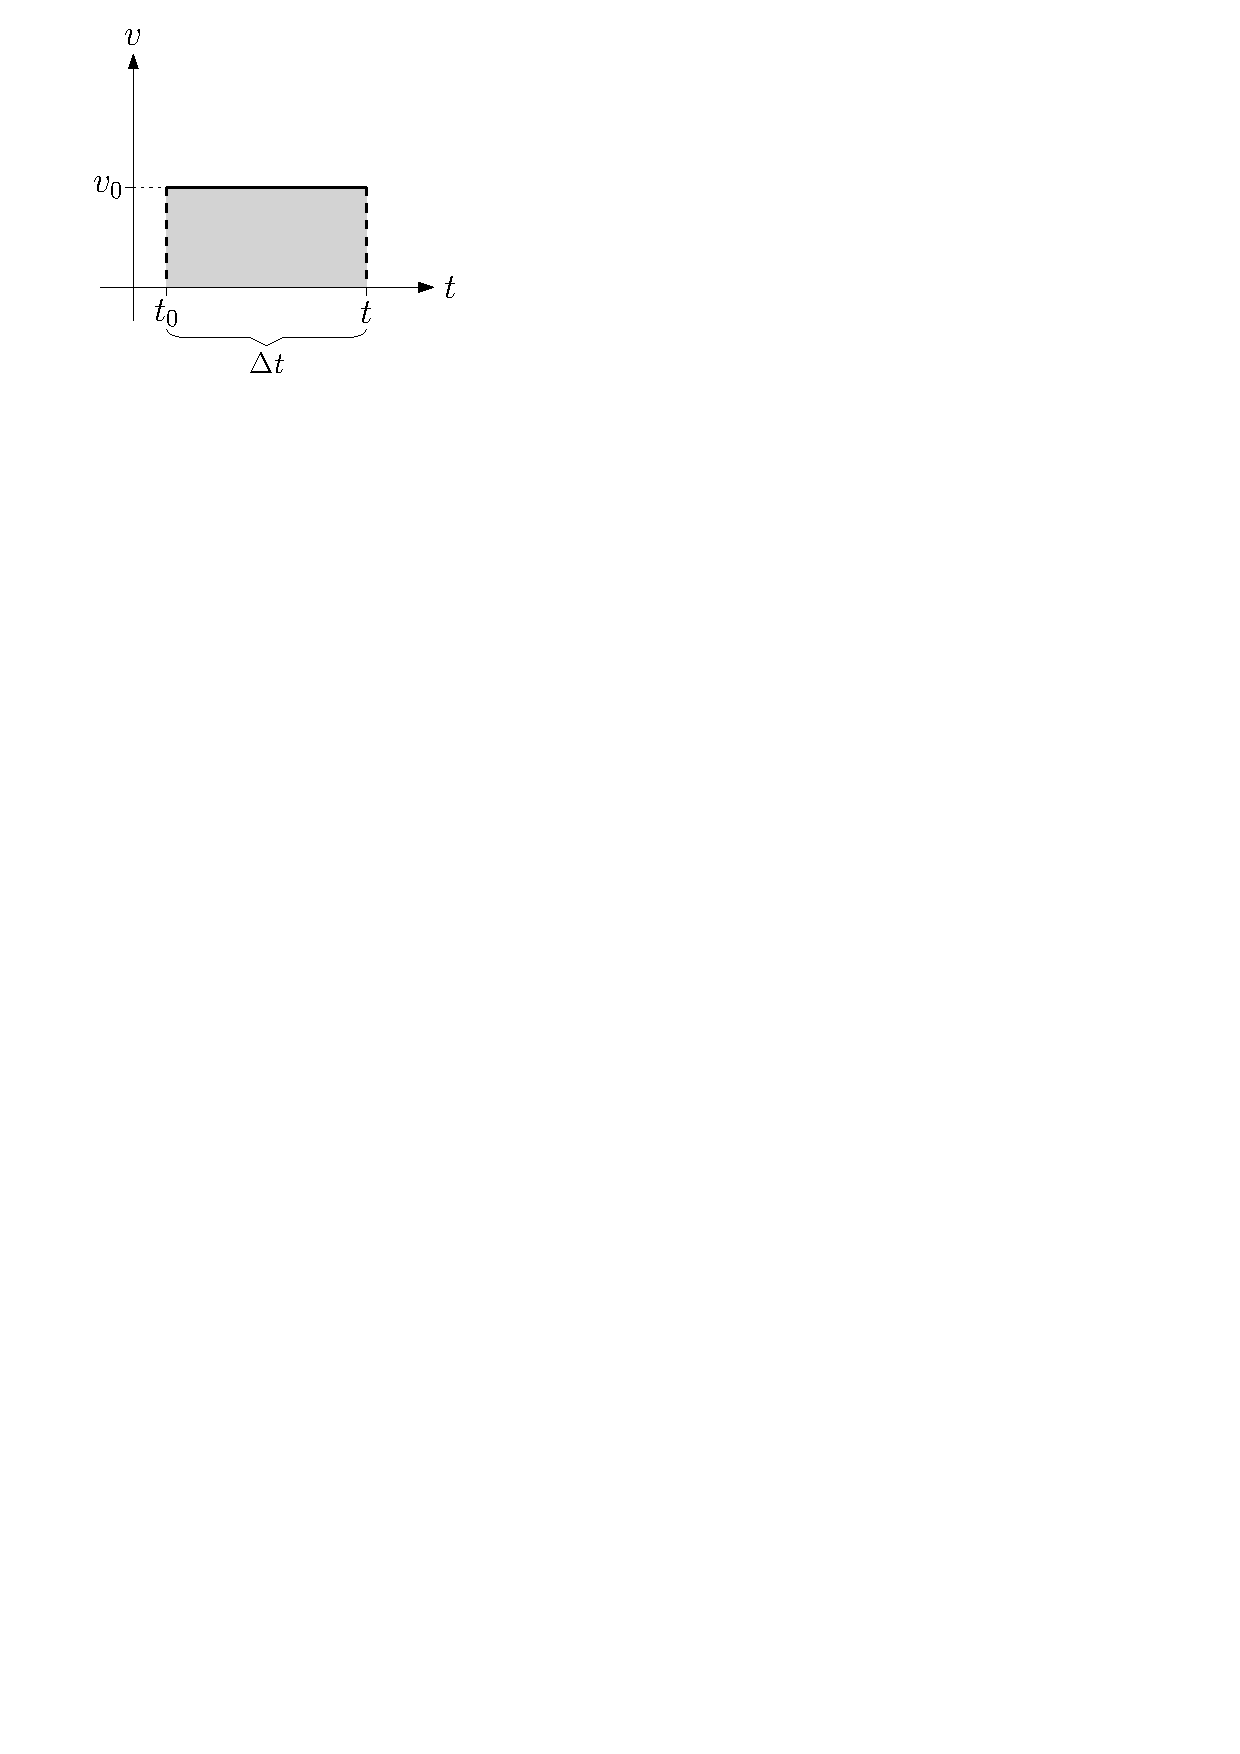
\includegraphics{img/area.pdf}
\caption{Gráfica de velocidad en función del tiempo para un MRU, el desplazamiento es el área marcada en gris}
\label{fig:area}
\end{figure}

La gráfica de la velocidad en función del tiempo para un MRUV se muestra en la Figura \ref{fig:area2}.

\begin{figure}[!h]
\centering
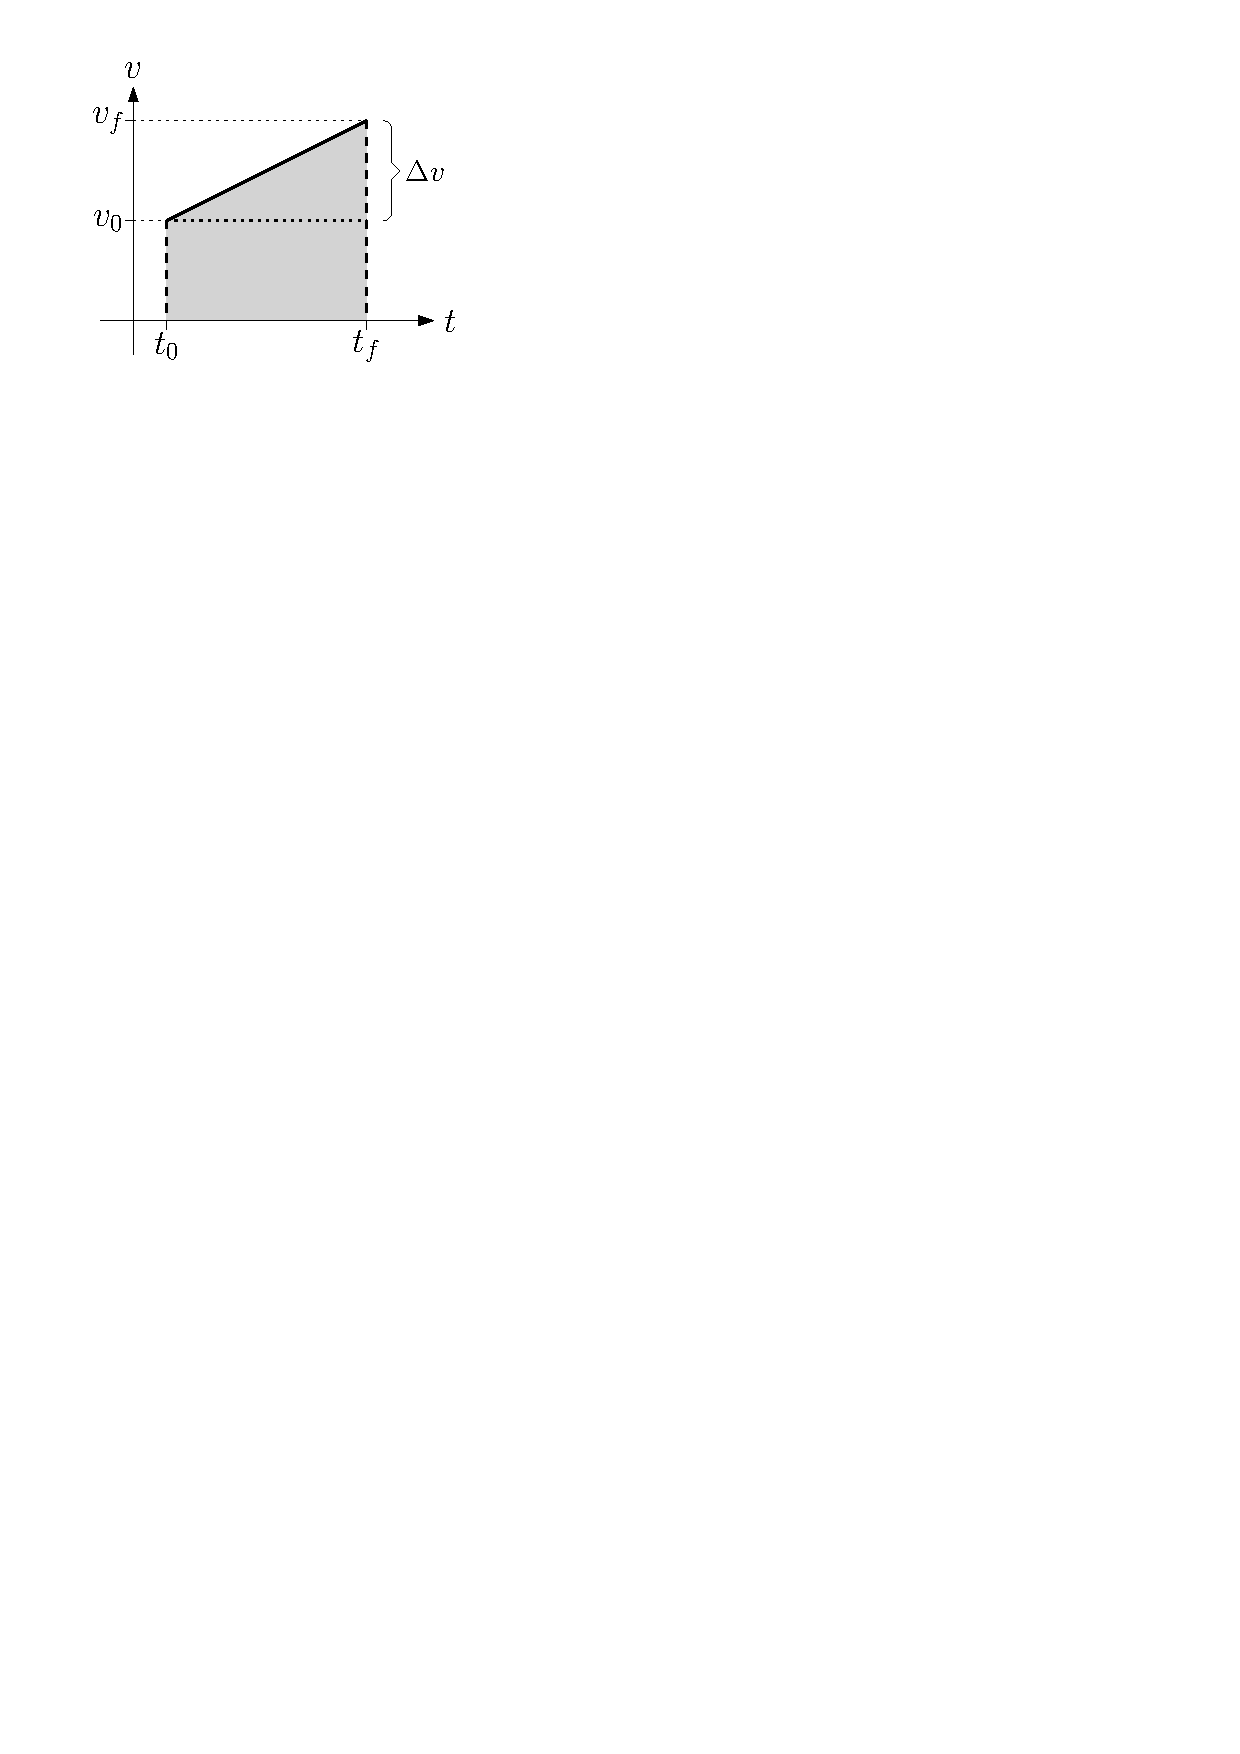
\includegraphics{img/area2.pdf}
\caption{Gráfica de velocidad en función del tiempo para un MRUV, el desplazamiento será el área en gris}
\label{fig:area2}
\end{figure}

Para calcular el área debajo de la curva podemos pensar que se compone de dos partes: un rectángulo y un triángulo.
\begin{eqnarray*}
\Delta x & = & \mbox{área }\square + \mbox{área } \triangle \\
& = & v_0(t-t_0) + \frac{1}{2} (v-v_0) (t-t_0) 
\end{eqnarray*}
Si multiplicamos y dividimos el último término por $(t-t_0)$
\begin{eqnarray*}
\Delta x & = & v_0(t-t_0) + \frac{1}{2} \overbrace{\frac{(v-v_0)}{\textcolor{red}{(t-t_0)}}}^{\displaystyle\textcolor{orange}{a}} (t-t_0) \textcolor{red}{(t-t_0)} \\
 & = & v_0 \Delta t  +  \frac{1}{2} a (\Delta t)^2 \\
x-x_0 & = & v_0 \Delta t + \frac{1}{2} a (\Delta t)^2
\end{eqnarray*}
De donde se obtiene:
\begin{center}
{\color{ForestGreen}  \boxed{\mathbold{x=x_0+v_0\Delta t+\frac{1}{2}a(\Delta t)^2}}}
\end{center}

Tal como planteamos originalmente, la expresión de $x-x_0$ tiene dos términos: $v_0\Delta t$ que ya aparecía en la ley de movimiento del MRU y el término $\frac{1}{2}a(\Delta t)^2$ que habla del desplazamiento adicional debido al cambio de velocidad. En otras palabras, una partícula que se mueve aumentando su velocidad se desplaza \textit{un poco más} que una que se mueve a velocidad constante.

Nótese que si $a=0$ estamos hablando de un MRU y la ecuación anterior se transforma en la que ya conocíamos:
$$x=x_0+v\Delta t$$

En muchas situaciones de interés, la \textit{Ley de movimiento del MRUV} se puede simplificar tomando $t_0=0$, y así nos queda $$x=x_0+v_0t+\frac{1}{2}at^2$$

\begin{mybox}{Para profundizar}

¿Por qué siempre el área bajo la curva de velocidad en función del tiempo es el desplazamiento? La idea de \textit{área bajo la curva} tiene muchas aplicaciones en Física. Si bien la justificación de esta idea excede el contenido de este curso, daremos una pequeña noción al respecto.

\begin{center}
\centering
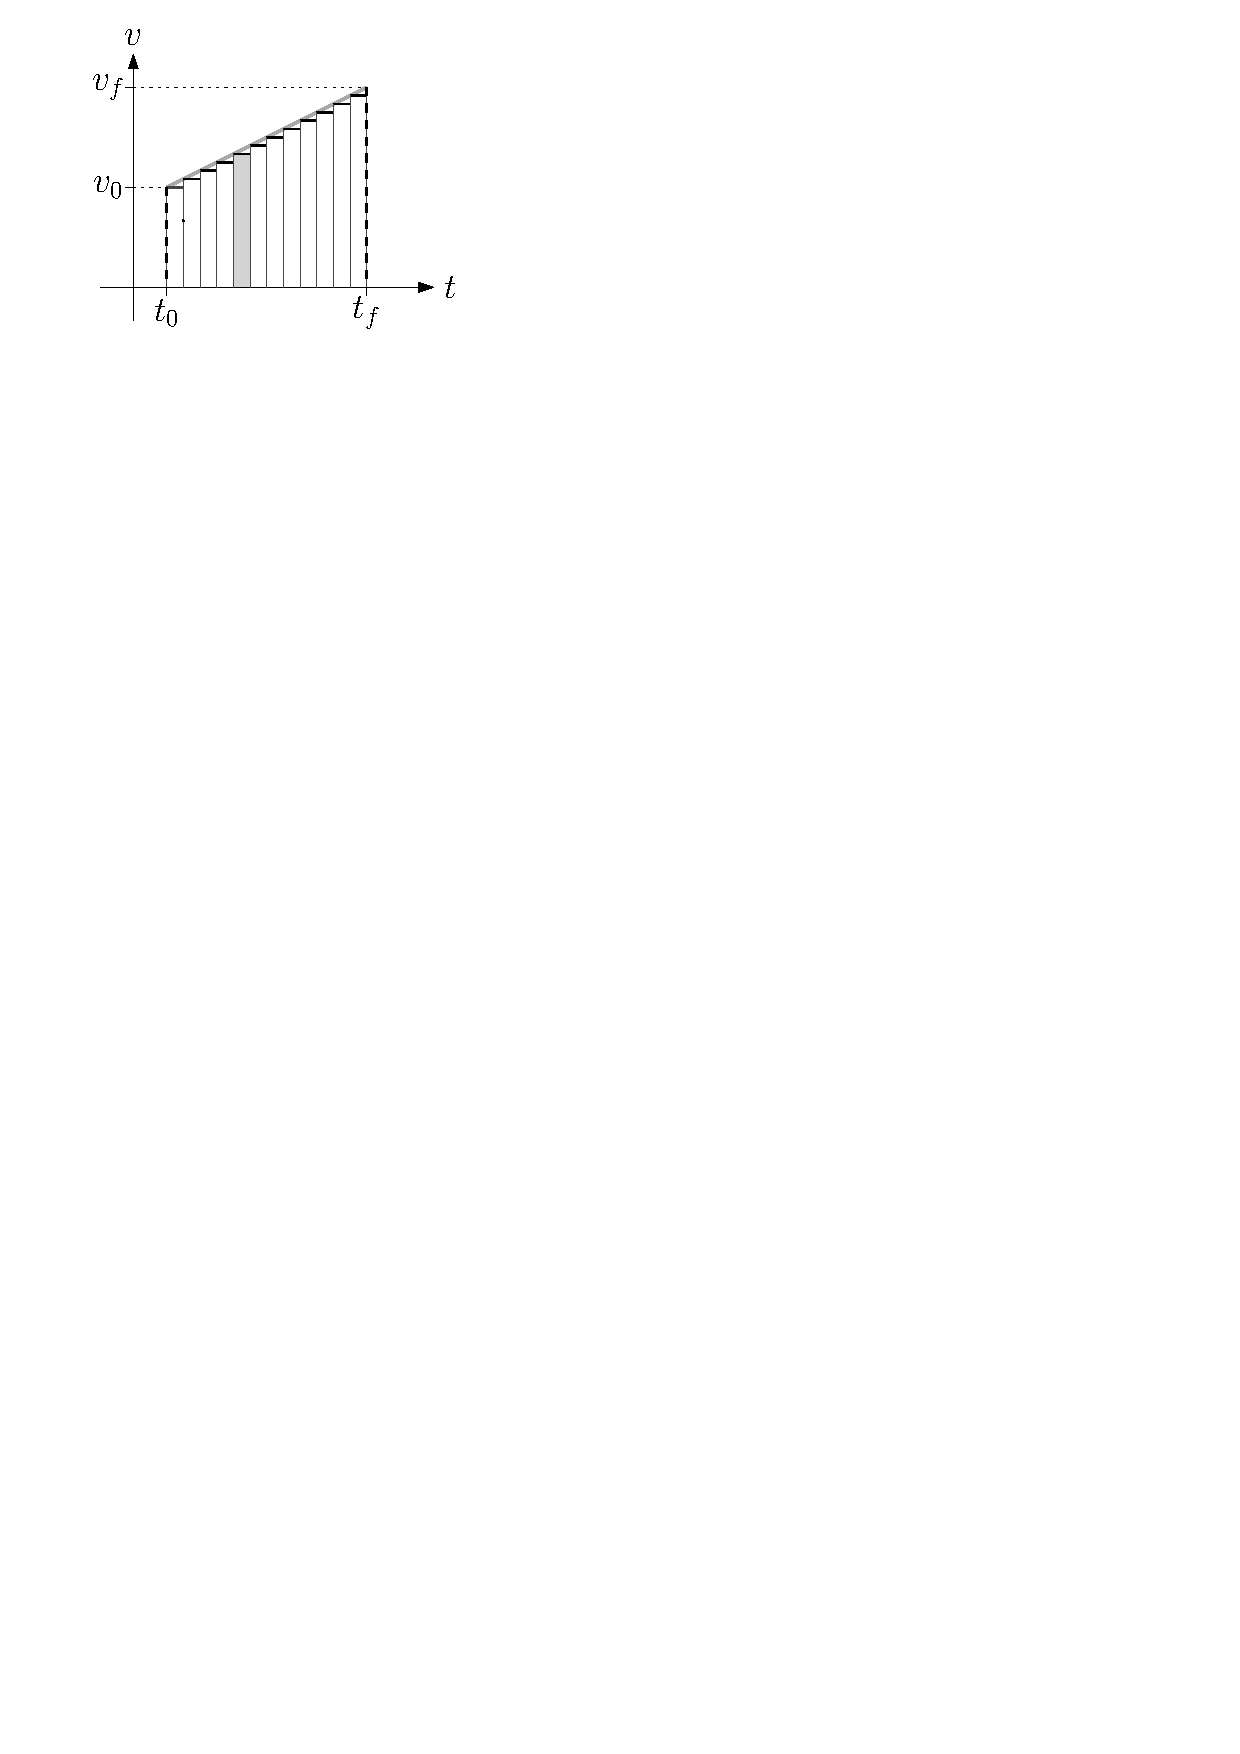
\includegraphics[scale=0.8]{img/integral.pdf}
\end{center}

Cuando la velocidad no es constante, se puede aproximar por pequeños tramos constantes. En otras palabras, podemos pensar que la partícula en cuestión se mueve con velocidad constante por pequeños intervalos de tiempo. Para cada uno de estos pequeños intervalos el desplazamiento es el área del rectángulo que queda determinado (como el que está indicado en gris en la gráfica de la Figura). Calcular el desplazamiento total equivale a sumar los desplazamientos correspondientes a cada intervalo, es decir, calcular el área bajo la curva.
\end{mybox}



Para obtener una expresión que nos permita calcular la velocidad de la partícula en función de su posición o de su desplazamiento, conociendo además su velocidad inicial y su aceleración y sin necesidad de calcular previamente el tiempo en la fórmula de posición, partimos de:
$$v = v_0 + a \Delta t$$
$$x = x_0 + v_0 \Delta t + \frac{1}{2}a(\Delta t)^2$$
Despejamos $\Delta t$ de la expresión de velocidad:
$$\Delta t = \frac{v - v_0}{a}$$
Reemplazamos en la expresión de $x$
$$x = x_0 + v_0 \frac{v - v_0}{a} + \frac{1}{2} a \frac{(v - v_0)^2}{a^2}$$
Y operando llegamos a 
\begin{center}
{\color{Magenta}  \boxed{\mathbold{v^2 = v_0^2 + 2 a \Delta x}}}
\end{center}

Vamos a ver cómo se analiza una situación de MRUV:

\begin{example}{Ejemplo}
%\item[] {\bf Ejemplo:}\\
    {\it El TGV (Train à Grande Vitesse, tren de gran velocidad, en francés) es un servicio interurbano de trenes de alta velocidad. Este tren ostenta el record de ser el tren con ruedas mas rapido del mundo, con una velocidad de $574,8 \si{km/h}$ (en condiciones de prueba). Un TGV parte de la estación, ¿cuál es la aceleración del tren, supuesta constante, si pasa de $0 \si{km/h}$ a $320 \si{km/h}$ (su velocidad operativa) en $7\si{min}$? ¿cuál es la distancia del tren a la estación a los $60\si{s}$, $120\si{s}$, $180\si{s}$ y $240\si{s}$?}
%\item[] 
    \tcblower
     {\sf {\bf Modelo:} Supondremos en este problema que el {\it TGV} es una partícula que se mueve en una trayectoria rectilínea con aceleración constante a determinar.}
  
Lo primero que hacemos es realizar un esquema de la situación física identificando los datos del problema, en este caso fijaremos el origen de coordenadas en la estación y tomaremos el sentido positivo hacia donde se mueve el tren (digamos: la derecha):
  \begin{center}
    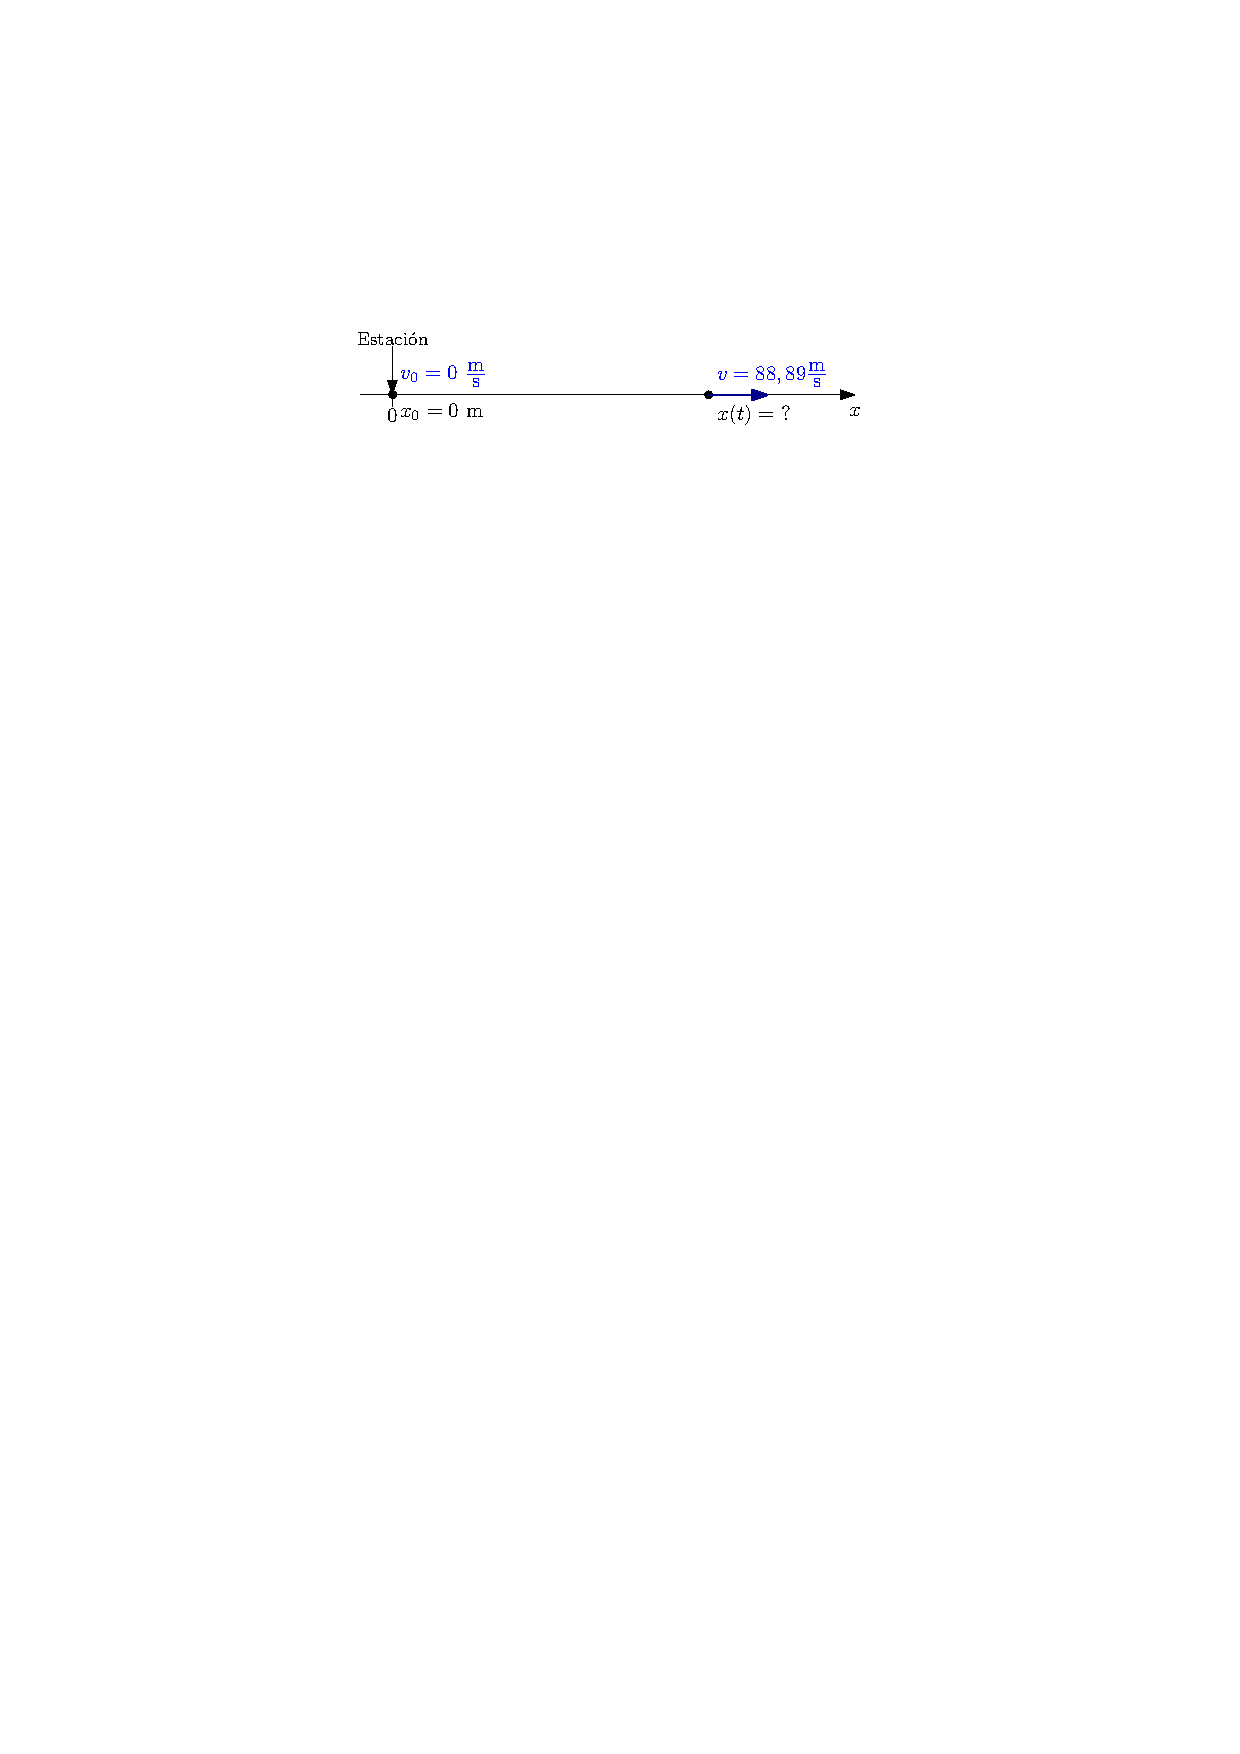
\includegraphics[]{img/tgv.pdf}
  \end{center}
  Con lo cual, podemos identificar los datos como:
  \begin{equation*}
	t_0=0\si{s}:
	\left\{
	\begin{array}{ccl}
	x_0 & = & 0\si{m}\\
	v_0 & = & 0\si{m/s}\\
	\end{array}
	\right.
	\quad
	t=7\si{min}\equiv 420 \si{s}
	\left\{
	\begin{array}{ccl}
	x & = & ?\\
	v & = & 320\sif{km}{h}\equiv 88,89 \sif{m}{s}\\
	\end{array}
	\right.
	\end{equation*}
  Nótese que dejamos indicado que la posición en el instante $t=420\si{s}$ es una incógnita. Con estos datos podemos calcular la aceleración del tren:
$$a=\frac{v-v_0}{t-t_0}=\frac{88,89\sif{m}{s}}{420\si{s}}=0,211\sif{m}{s$^2$}$$
  
  Teniendo la aceleración, podemos utilizarla junto con los datos para calcular la posición del tren respecto a la estación en los instantes pedidos (recordemos que $t_0=0\si{s}$, $x_0=0\si{m}$ y $v_0=0\si{m/s}$):
  $$60\si{s}:\quad x = \cancel{x_0} + \cancel{v_0t} + \frac{1}{2}at^2= \frac{1}{2} \cdot 0,211\sif{m}{s$^2$} \cdot (60\si{s})^2  = 379,8 \si{m}$$
  $$120\si{s}:\quad x = \cancel{x_0} + \cancel{v_0t}+ \frac{1}{2}at^2 = \frac{1}{2} \cdot 0,211\sif{m}{s$^2$} \cdot (120\si{s})^2 = 1519,2\si{m}$$
  $$180\si{s}:\quad x = \cancel{x_0} + \cancel{v_0t}+ \frac{1}{2}at^2 = \frac{1}{2} \cdot 0,211\sif{m}{s$^2$} \cdot (180\si{s})^2 = 3418,2\si{m}$$
  $$240\si{s}:\quad x = \cancel{x_0} + \cancel{v_0t}+ \frac{1}{2}at^2 = \frac{1}{2} \cdot 0,211\sif{m}{s$^2$} \cdot (240\si{s})^2 = 6076.8\si{m}$$
\end{example}

Al igual que hicimos para el MRU, la información obtenida se puede llevar a una gráfica de \textbf{posición en función del tiempo} $\mathbold{x=x(t)}$.

\begin{figure}[!h]
  \centering
  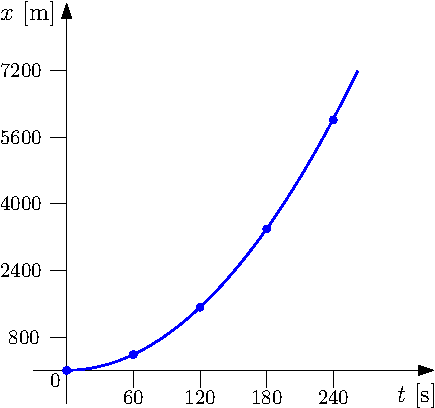
\includegraphics[scale=1]{img/x_tgv.pdf}
  \caption{\label{fig:MRUV} Gráfica típica $x=x(t)$ de un MRUV.}
\end{figure}

Se deja como ejercicio para el lector realizar la gráfica de \textbf{velocidad en función del tiempo} $\mathbold{v=v(t)}$.

La gráfica de posición en función del tiempo para un MRUV será, como en el ejemplo anterior, una \textbf{parábola}. ¿Qué información se puede extraer de este tipo de gráficas? La Figura \ref{fig:rectatangente} presenta una gráfica de posición en función del tiempo (también llamada \textbf{posición versus tiempo}, $\mathbold{x\ \mathbf{vs}\ t}$).

\begin{figure}[!h]
  \centering
  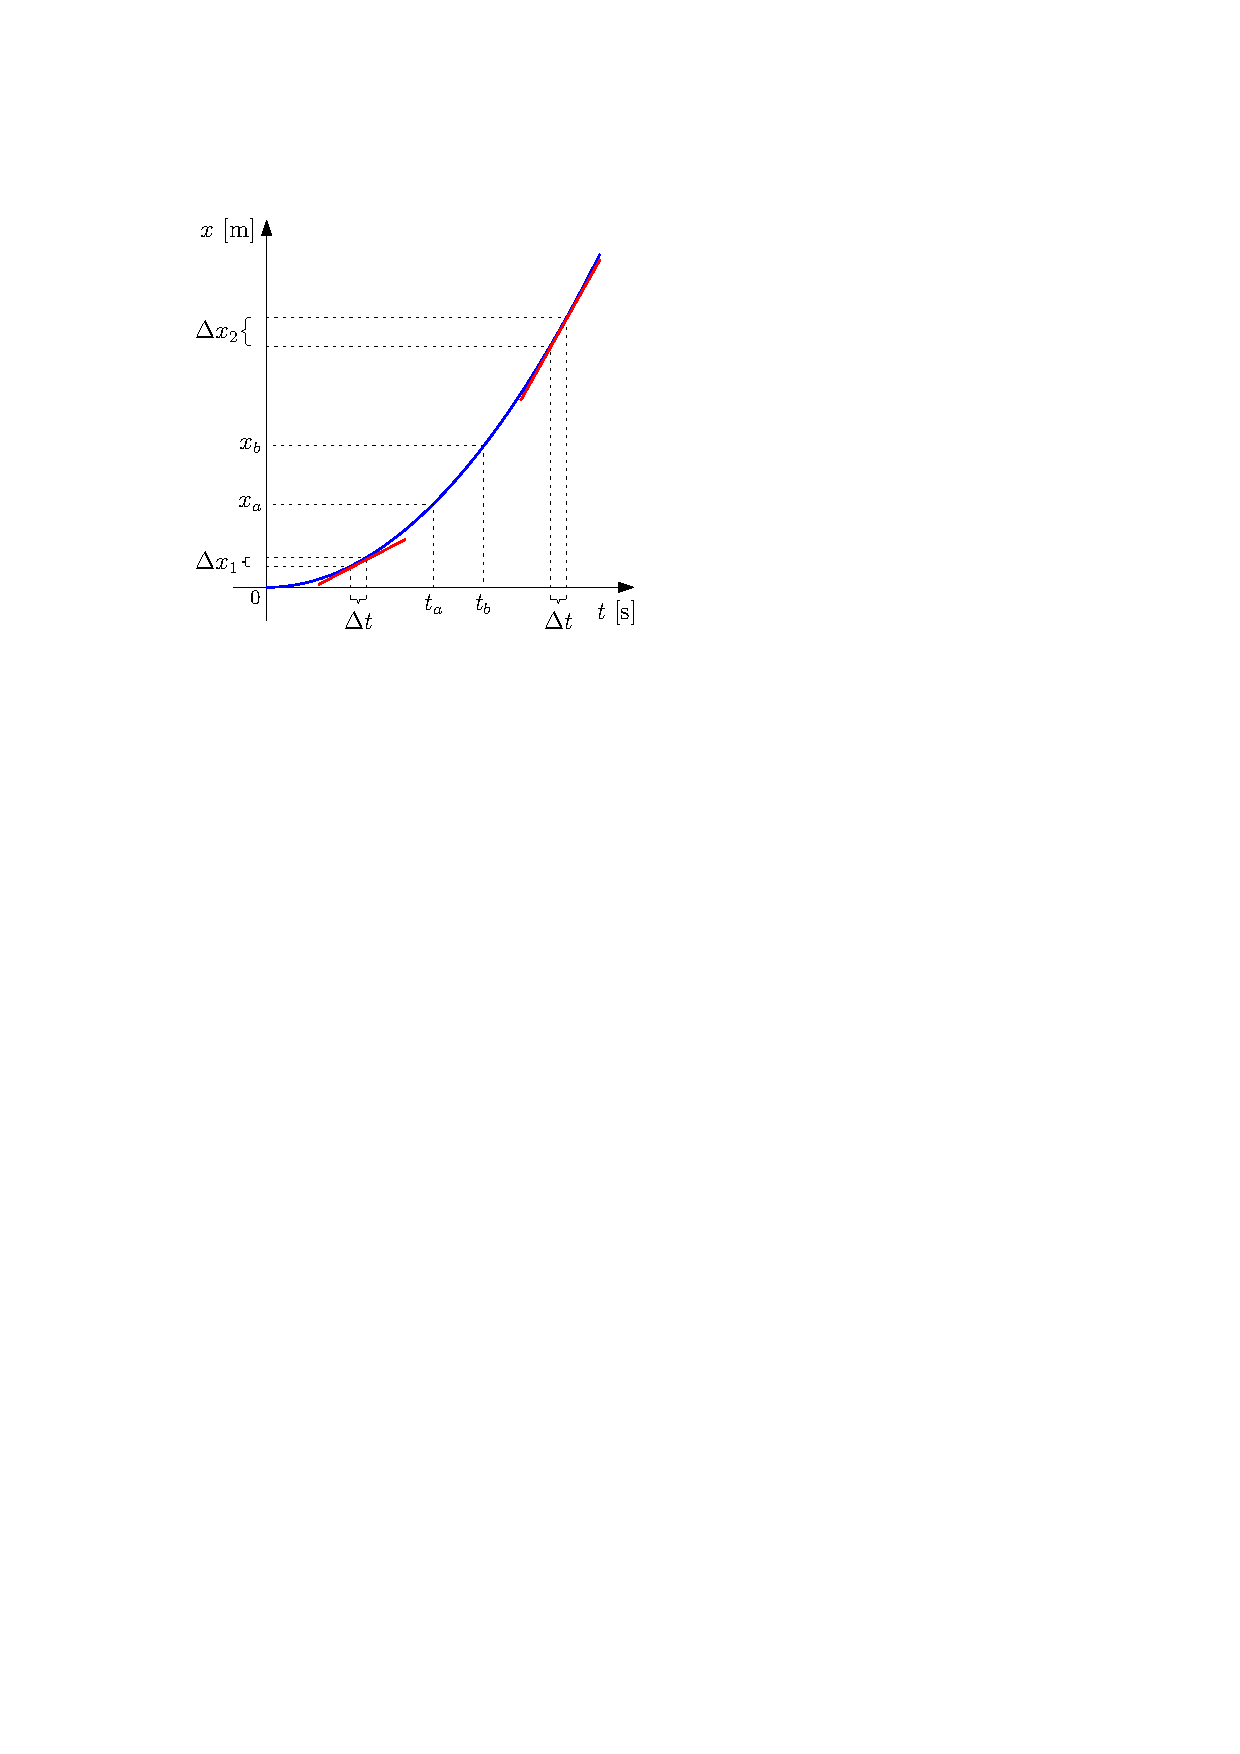
\includegraphics[scale=1]{img/rectatangente.pdf}
  \caption{\label{fig:rectatangente} Gráfica típica x=x(t) de un MRUV.}
\end{figure}

En primer lugar, podemos decir que la partícula parte de $x_0 = 0$ (ya que en $t=0$, $x=0$), y se mueve en el sentido tomado como positivo: si tomamos un instante de tiempo $t_a$ y un instante posterior $t_b$ (en el ejemplo del TGV sería por ejemplo $t_a =120\si{s}$ y $t_b=180\si{s}$), vemos que la partícula está primero en $x_a$ y luego pasa por $x_b$, y que $x_b > x_a$.

Podemos darnos cuenta que la rapidez va aumentando porque si tomamos dos pequeños intervalos de tiempo iguales (en el eje horizontal), vemos que en el intervalo que está a la derecha (es decir, que ocurre luego), el desplazamiento $\Delta x_2$ es mayor que el desplazamiento $\Delta x_1$. En otras palabras, es la pendiente de la recta tangente a la curva (en \textcolor{red}{rojo}) la que nos dice qué tan \textit{rápido} se mueve la partícula: mientras más \textit{empinada} la recta tangente, mayor es la velocidad.

A partir de la gráfica también podemos determinar que la partícula parte del reposo ($v_0=0$) ya que al principio, la recta tangente es horizontal y no tiene pendiente.

Analicemos un caso más agregando las gráficas de velocidad y aceleración en función del tiempo.

\begin{example}{Ejemplo}
%\item[] {\bf Ejemplo:}\\
    {\it Un esquiador en el Cerro Catedral (San Carlos Bariloche) desacelera hasta detenerse en una superficie horizontal luego de haber descendido por la pista. Bosquejar las gráficas de $x(t)$, $v(t)$ y $a(t)$}
%\item[] :
\tcblower
Como no tenemos más datos, fijamos un sistema de referencia arbitrario y diremos que el esquiador está en una posición inicial $x_0$ positiva cualquiera. 

  \begin{center}
    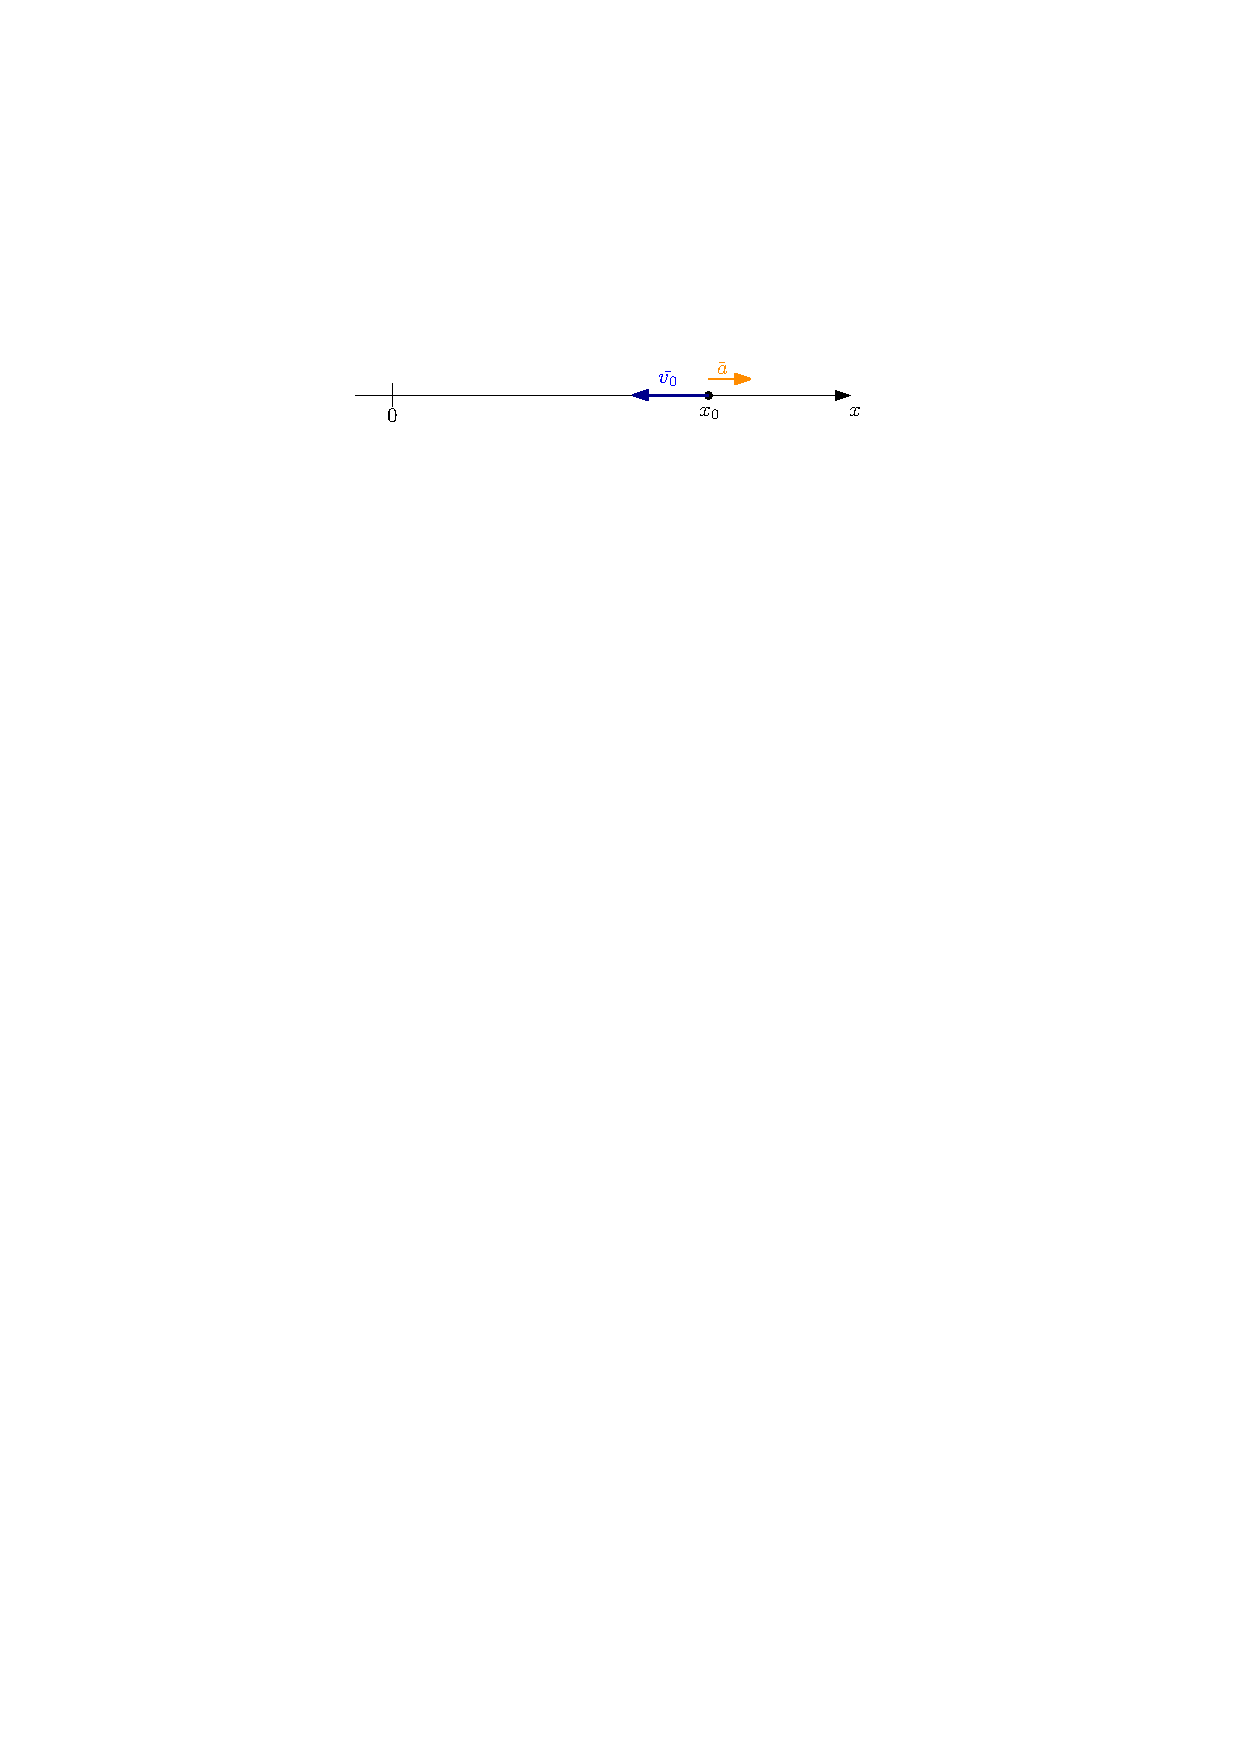
\includegraphics[]{img/esquiador.pdf}
  \end{center}

La velocidad inicial es negativa para el sistema de referencia adoptado y va hasta cero (disminuye su módulo). La aceleración es siempre positiva para el sistema de referencia. Según el esquema el esquiador se mueve acercándose al origen de coordenadas. En $t^*$ la velocidad se hace cero y el esquiador se detiene (la tangente a la curva de posición es horizontal).

  \begin{center}
    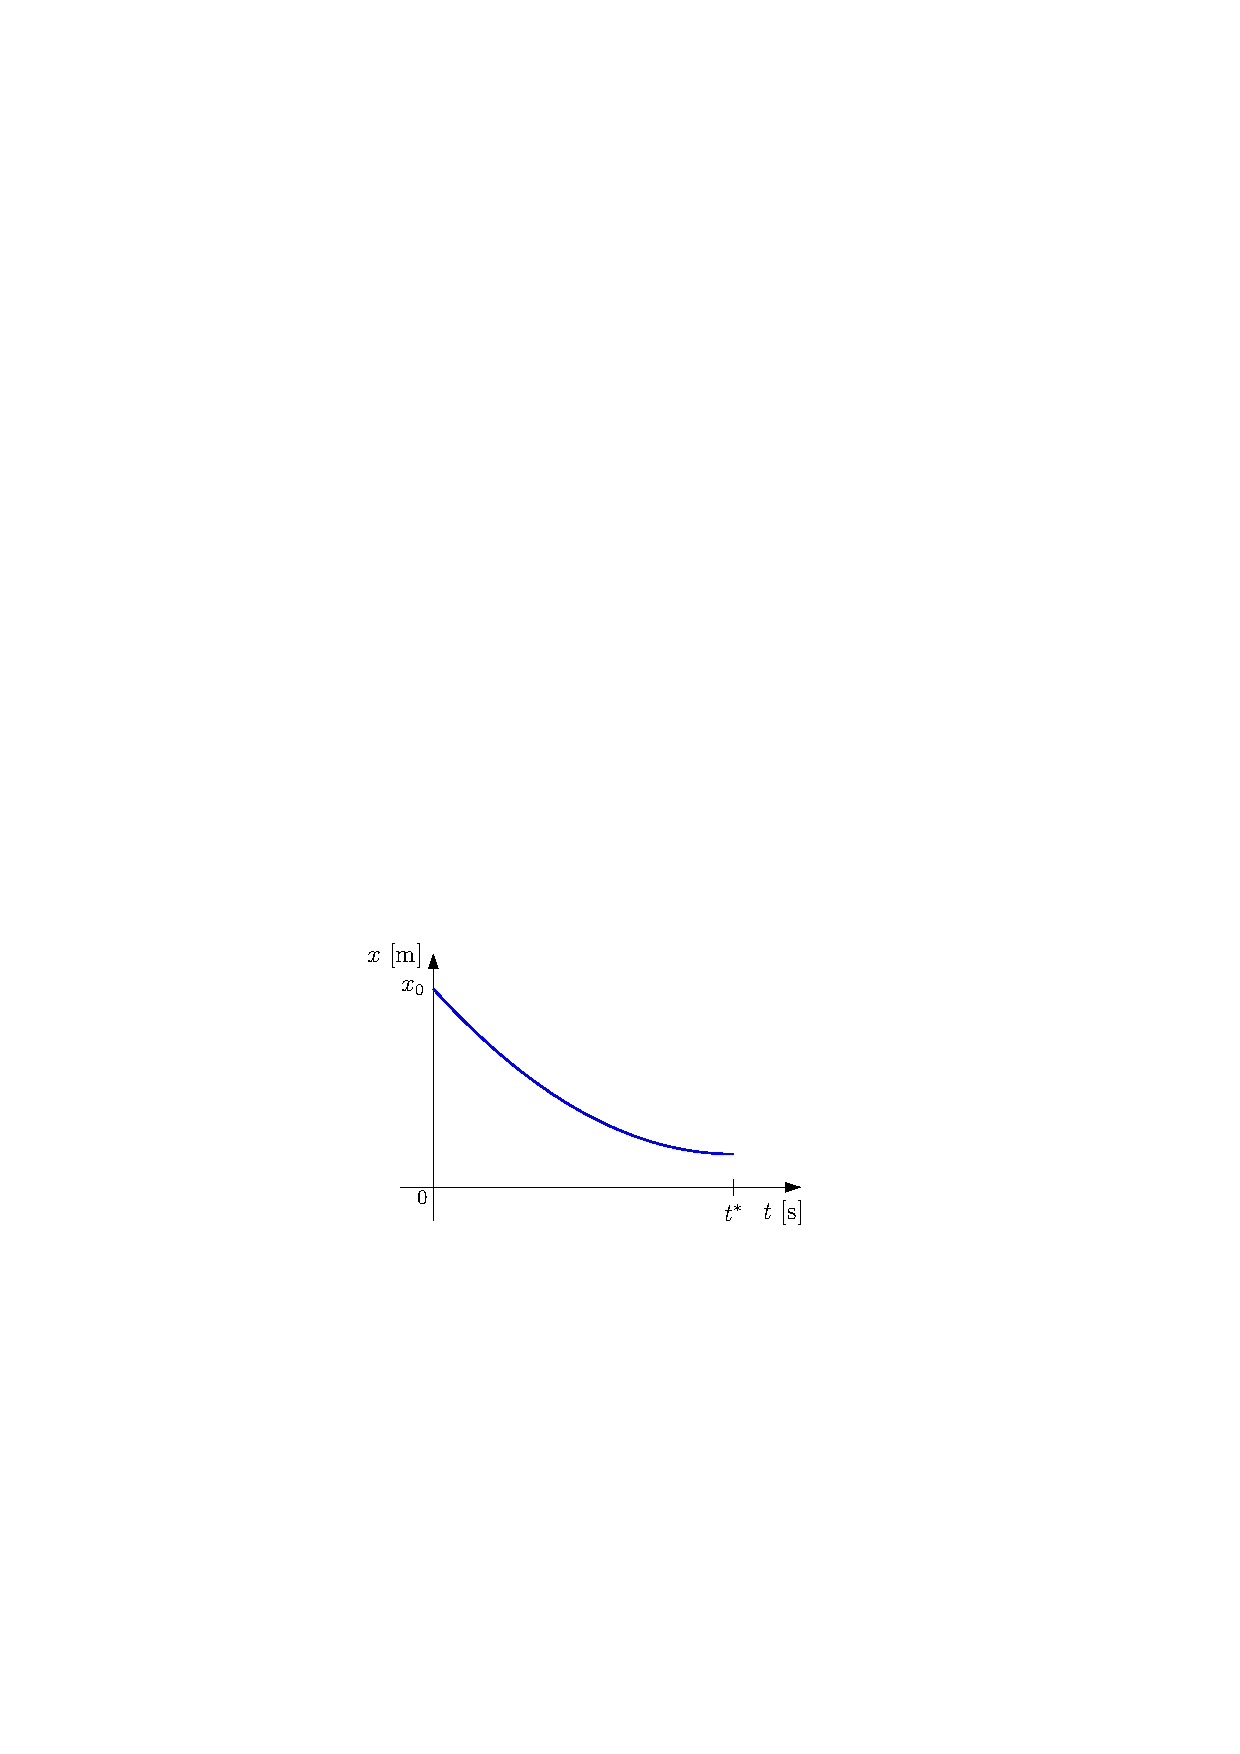
\includegraphics[]{img/plot2a.pdf}
    
    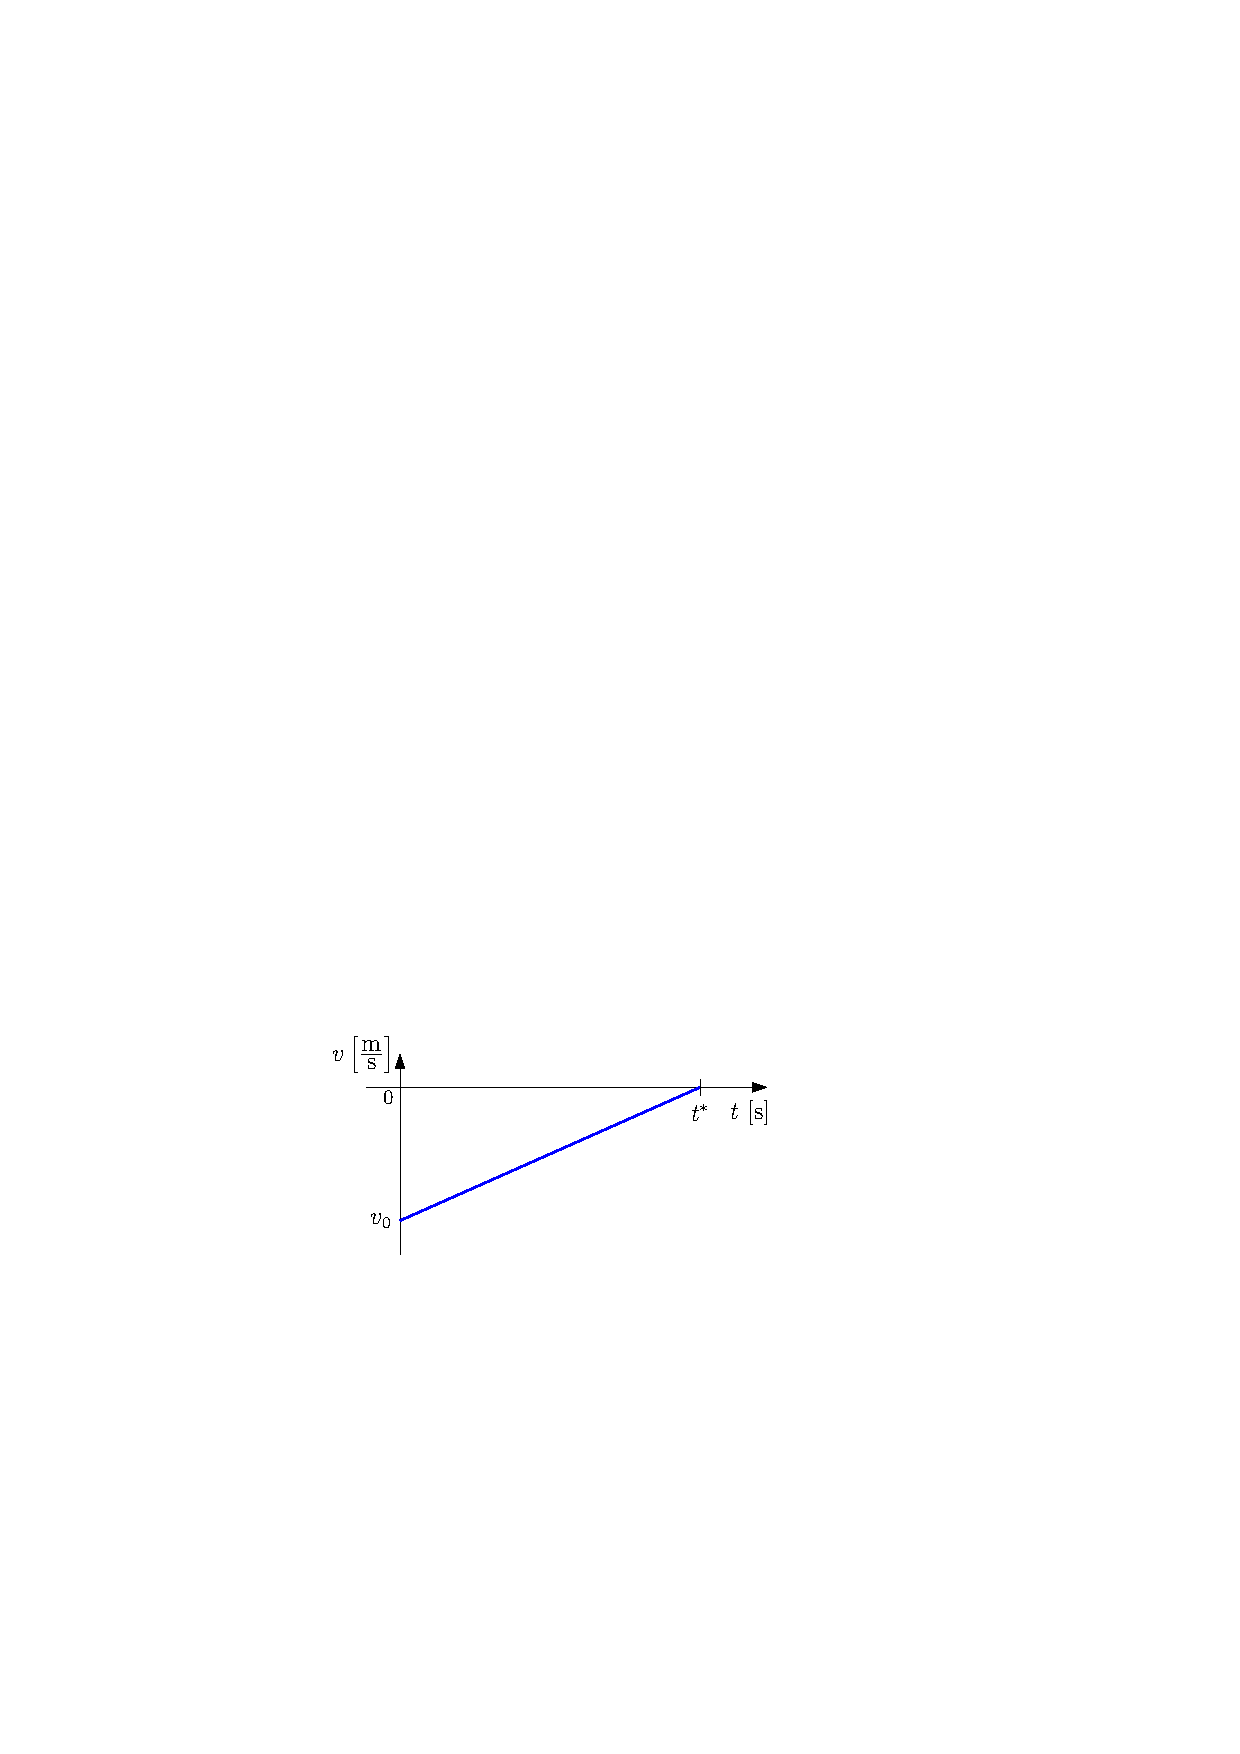
\includegraphics[]{img/plot2b.pdf}
    
    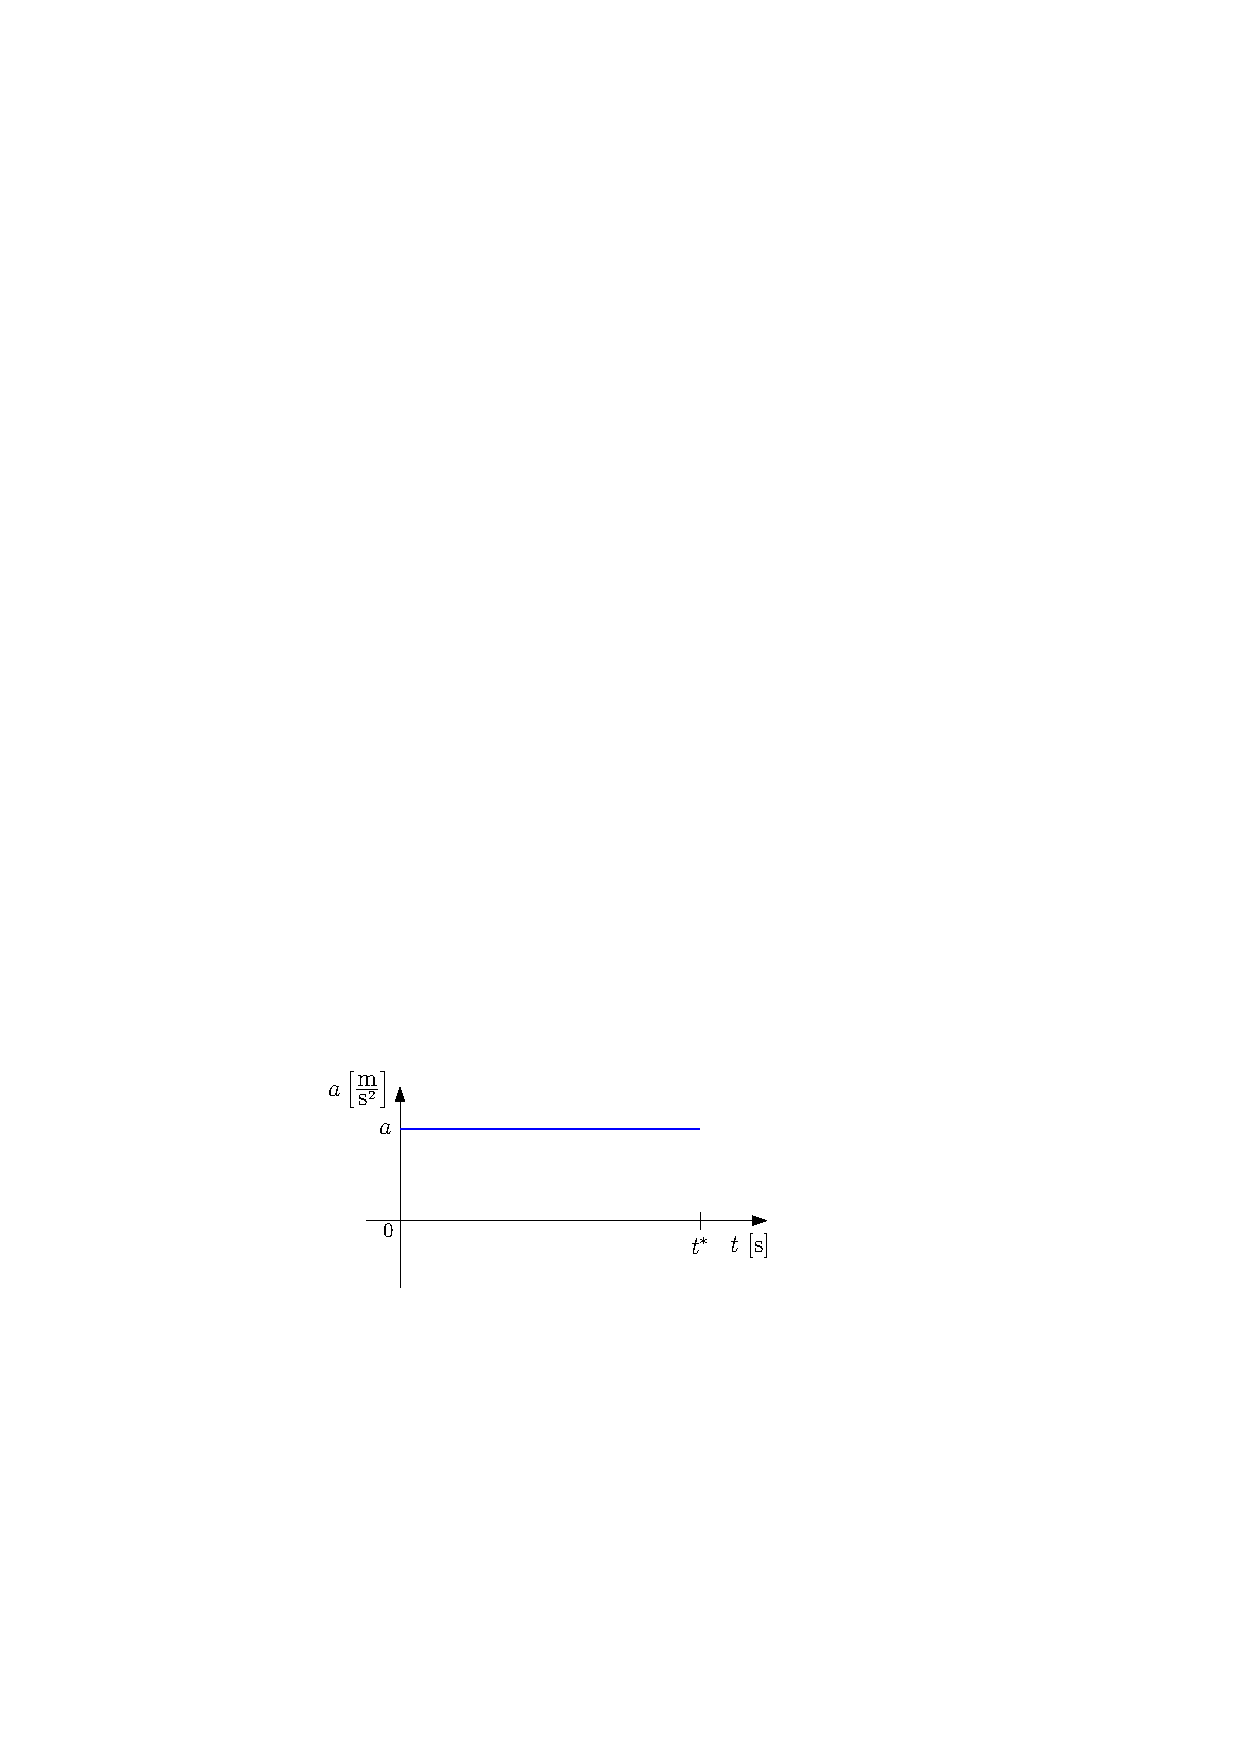
\includegraphics[]{img/plot2c.pdf}
  \end{center}
\end{example}


\begin{comprension}
  \noindent
  {\bf Primero}  Analiza las siguientes gráficas:
  \begin{center}
    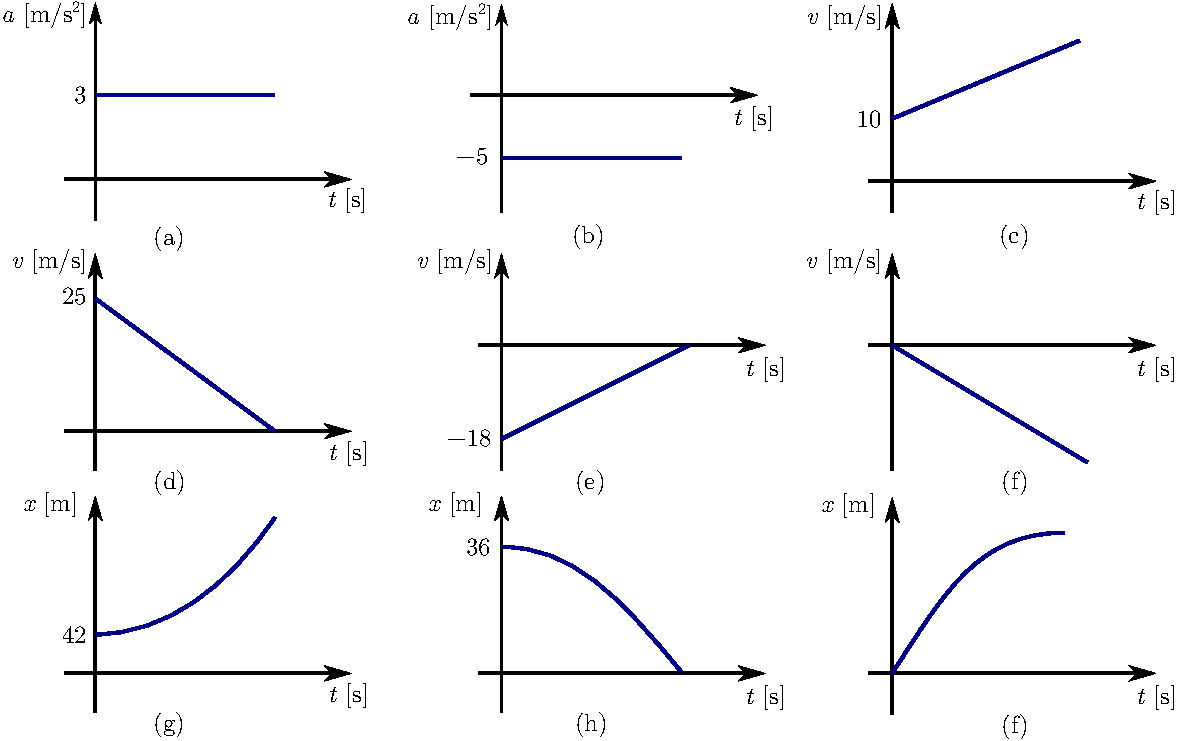
\includegraphics[width=0.9\textwidth]{img/analisisMRUV.pdf}
  \end{center}

 \noindent
  {\bf Segundo} ¿Pueden la gráfica (b) y la (c) pertenecer a un mismo movimiento? ¿La (d) y la (f)? Explica.
\end{comprension}
